\section{Representação do Jogo}

\begin{frame}
\frametitle{\secname\\\emph{Renée v Peter}}
Exemplo de jogo
\begin{itemize}
	\item Dois jogadores: \textbf{\emph{Renée}} e \textbf{\emph{Peter}}
	\pause
	\item Três cartas: Rei (\textbf{\emph{K}}), Dez (\textbf{\emph{T}}) e Dois (\textbf{\emph{D}})
	\pause
	\item[\emph{R}] Escolhe uma carta
	\pause
	\item[\emph{P}] Adivinha se \emph{\textbf{Alta}} (\emph{K}) ou \emph{\textbf{Baixa}} (\emph{D})
	\pause
	\begin{itemize}
		\item[\emph{P}] erra, \emph{R} ganha 2
		\pause
		\item[\emph{P}] acerta, \emph{R} perde 3
	\end{itemize}
	\pause
	\item No caso $T$
	\pause
	\begin{itemize}
		\item[\emph{Baixa}] \emph{R} ganha 1
		\pause
		\item[\emph{Alta}] \emph{R} escolhe outra carta
	\end{itemize}
	\pause
	\begin{itemize}
		\item[\emph{P}] erra, \emph{R} ganha 3
		\pause
		\item[\emph{P}] acerta, \emph{R} perde 1
	\end{itemize}
\end{itemize}
\end{frame}

\subsection{Forma Extensa}
\begin{frame}
\frametitle{Forma Extensa\\Vez de \emph{Renée}}
\begin{figure}[ht]
	\centering
	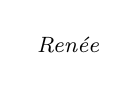
\begin{tikzpicture}
	  [
	    grow                    = down,
	    edge from parent/.style = {draw, -latex},
	    every node/.style       = {font=\footnotesize},
	    sloped,
		level 1/.style			= {
			sibling distance=2.5cm,
			level distance=1cm
		},
		level 2/.style			= {
			sibling distance=1.5cm,
			level distance=1.5cm
		},
		level 3/.style			= {
			sibling distance=2cm,
			level distance=1cm
		},
		level 4/.style			= {
			sibling distance=1.5cm,
			level distance=1.5cm
		}
		]
		\node {\emph{Renée}};
%		child {
%			node (P1){}{%\emph{Peter}} {
%				child {
%					node {}%{\textbf{-3}}
%					edge from parent node [above] {}%{\emph{Alta}}
%				}
%				child {
%					node {}%{\textbf{2}}
%					edge from parent node [above] {}%{\emph{Baixa}}
%				}
%			}
			% edge from parent node [above] {$K$}
%		}
%		child {
%			node (P2) {}{%\emph{Peter}} {
%				child {
%					node (R) {}{%\emph{Renée}} {
%						child {
%							node (P21) {}{%\emph{Peter}} {
%							child {
%								node {}%{\textbf{-1}}
%								% edge from parent node [above] {}%{\emph{Alta}}
%							}
%							child {
%								node {}%{\textbf{3}}
%								% edge from parent node [above] {}%{\emph{Baixa}}
%							}
%							}
%							% edge from parent node [above] {$K$}
%						}
%						child {
%							node (P22) {}{%\emph{Peter}} {
%							child {
%								node {}%{\textbf{3}}
%								% edge from parent node [above] {}%{\emph{Alta}}
%							}
%							child {
%								node {}%{\textbf{-1}}
%								% edge from parent node [above] {}%{\emph{Baixa}}
%							}
%							}
%							% edge from parent node [above] {$D$}
%						}
%					}
%					% edge from parent node [above] {}%{\emph{Alta}}
%				}
%				child {
%				node {}%{\textbf{1}}
%				% edge from parent node [above] {}%{\emph{Baixa}}
%				}
%			}
%			% edge from parent node [above] {$T$}
%		}
%		child {
%			node (P3) {}{%\emph{Peter}} {
%				child {
%					node {}%{\textbf{2}}
%					% edge from parent node [above] {}%{\emph{Alta}}
%				}
%				child {
%					node {}%{\textbf{-3}}
%					% edge from parent node [above] {}%{\emph{Baixa}}
%				}
%			}
			% edge from parent node [above] {$D$}
%		};
%		\draw[thick, rounded corners] ($(P1.north west)+(-0.1,-0.1)$) rectangle ($(P3.south east)+(0.1,+0.1)$);
%		\draw[thick, rounded corners] ($(P21.north west)+(-0.1,-0.1)$) rectangle ($(P22.south east)+(0.1,+0.1)$);
	\end{tikzpicture}
\end{figure}
\end{frame}

\begin{frame}
\frametitle{Forma Extensa\\Opções de \emph{Renée}}
\begin{figure}[ht]
	\centering
	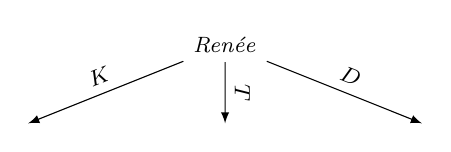
\begin{tikzpicture}
	  [
	    grow                    = down,
	    edge from parent/.style = {draw, -latex},
	    every node/.style       = {font=\footnotesize},
	    sloped,
		level 1/.style			= {
			sibling distance=2.5cm,
			level distance=1cm
		},
		level 2/.style			= {
			sibling distance=1.5cm,
			level distance=1.5cm
		},
		level 3/.style			= {
			sibling distance=2cm,
			level distance=1cm
		},
		level 4/.style			= {
			sibling distance=1.5cm,
			level distance=1.5cm
		}
		]
		\node {\emph{Renée}}
		child {
%			node (P1){}{%\emph{Peter}} {
%				child {
%					node {}%{\textbf{-3}}
%					edge from parent node [above] {}%{\emph{Alta}}
%				}
%				child {
%					node {}%{\textbf{2}}
%					edge from parent node [above] {}%{\emph{Baixa}}
%				}
%			}
			edge from parent node [above] {$K$}
		}
		child {
%			node (P2) {}{%\emph{Peter}} {
%				child {
%					node (R) {}{%\emph{Renée}} {
%						child {
%							node (P21) {}{%\emph{Peter}} {
%							child {
%								node {}%{\textbf{-1}}
%								% edge from parent node [above] {}%{\emph{Alta}}
%							}
%							child {
%								node {}%{\textbf{3}}
%								% edge from parent node [above] {}%{\emph{Baixa}}
%							}
%							}
%							% edge from parent node [above] {$K$}
%						}
%						child {
%							node (P22) {}{%\emph{Peter}} {
%							child {
%								node {}%{\textbf{3}}
%								% edge from parent node [above] {}%{\emph{Alta}}
%							}
%							child {
%								node {}%{\textbf{-1}}
%								% edge from parent node [above] {}%{\emph{Baixa}}
%							}
%							}
%							% edge from parent node [above] {$D$}
%						}
%					}
%					% edge from parent node [above] {}%{\emph{Alta}}
%				}
%				child {
%				node {}%{\textbf{1}}
%				% edge from parent node [above] {}%{\emph{Baixa}}
%				}
%			}
			edge from parent node [above] {$T$}
		}
		child {
%			node (P3) {}{%\emph{Peter}} {
%				child {
%					node {}%{\textbf{2}}
%					% edge from parent node [above] {}%{\emph{Alta}}
%				}
%				child {
%					node {}%{\textbf{-3}}
%					% edge from parent node [above] {}%{\emph{Baixa}}
%				}
%			}
			edge from parent node [above] {$D$}
		};
%		\draw[thick, rounded corners] ($(P1.north west)+(-0.1,-0.1)$) rectangle ($(P3.south east)+(0.1,+0.1)$);
%		\draw[thick, rounded corners] ($(P21.north west)+(-0.1,-0.1)$) rectangle ($(P22.south east)+(0.1,+0.1)$);
	\end{tikzpicture}
\end{figure}
\end{frame}

\begin{frame}
\frametitle{Forma Extensa\\Vez de \emph{Peter}}
\begin{figure}[ht]
	\centering
	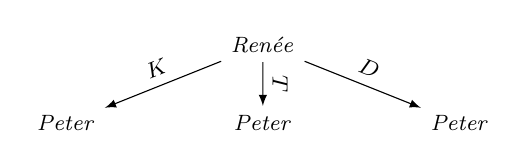
\begin{tikzpicture}
	  [
	    grow                    = down,
	    edge from parent/.style = {draw, -latex},
	    every node/.style       = {font=\footnotesize},
	    sloped,
		level 1/.style			= {
			sibling distance=2.5cm,
			level distance=1cm
		},
		level 2/.style			= {
			sibling distance=1.5cm,
			level distance=1.5cm
		},
		level 3/.style			= {
			sibling distance=2cm,
			level distance=1cm
		},
		level 4/.style			= {
			sibling distance=1.5cm,
			level distance=1.5cm
		}
		]
		\node {\emph{Renée}}
		child {
			node (P1){\emph{Peter}} {
%				child {
%					node {}%{\textbf{-3}}
%					edge from parent node [above] {}%{\emph{Alta}}
%				}
%				child {
%					node {}%{\textbf{2}}
%					edge from parent node [above] {}%{\emph{Baixa}}
%				}
			}
			edge from parent node [above] {$K$}
		}
		child {
			node (P2) {\emph{Peter}} {
%				child {
%					node (R) {}{%\emph{Renée}} {
%						child {
%							node (P21) {}{%\emph{Peter}} {
%							child {
%								node {}%{\textbf{-1}}
%								% edge from parent node [above] {}%{\emph{Alta}}
%							}
%							child {
%								node {}%{\textbf{3}}
%								% edge from parent node [above] {}%{\emph{Baixa}}
%							}
%							}
%							% edge from parent node [above] {$K$}
%						}
%						child {
%							node (P22) {}{%\emph{Peter}} {
%							child {
%								node {}%{\textbf{3}}
%								% edge from parent node [above] {}%{\emph{Alta}}
%							}
%							child {
%								node {}%{\textbf{-1}}
%								% edge from parent node [above] {}%{\emph{Baixa}}
%							}
%							}
%							% edge from parent node [above] {$D$}
%						}
%					}
%					% edge from parent node [above] {}%{\emph{Alta}}
%				}
%				child {
%				node {}%{\textbf{1}}
%				% edge from parent node [above] {}%{\emph{Baixa}}
%				}
			}
			edge from parent node [above] {$T$}
		}
		child {
			node (P3) {\emph{Peter}} {
%				child {
%					node {}%{\textbf{2}}
%					% edge from parent node [above] {}%{\emph{Alta}}
%				}
%				child {
%					node {}%{\textbf{-3}}
%					% edge from parent node [above] {}%{\emph{Baixa}}
%				}
			}
			edge from parent node [above] {$D$}
		};
%		\draw[thick, rounded corners] ($(P1.north west)+(-0.1,-0.1)$) rectangle ($(P3.south east)+(0.1,+0.1)$);
%		\draw[thick, rounded corners] ($(P21.north west)+(-0.1,-0.1)$) rectangle ($(P22.south east)+(0.1,+0.1)$);
	\end{tikzpicture}
\end{figure}
\end{frame}

\begin{frame}
\frametitle{Forma Extensa\\Conjunto de Informação}
\begin{figure}[ht]
	\centering
	\begin{tikzpicture}
	  [
	    grow                    = down,
	    edge from parent/.style = {draw, -latex},
	    every node/.style       = {font=\footnotesize},
	    sloped,
		level 1/.style			= {
			sibling distance=2.5cm,
			level distance=1cm
		},
		level 2/.style			= {
			sibling distance=1.5cm,
			level distance=1.5cm
		},
		level 3/.style			= {
			sibling distance=2cm,
			level distance=1cm
		},
		level 4/.style			= {
			sibling distance=1.5cm,
			level distance=1.5cm
		}
		]
		\node {\emph{Renée}}
		child {
			node (P1){\emph{Peter}} {
%				child {
%					node {}%{\textbf{-3}}
%					edge from parent node [above] {}%{\emph{Alta}}
%				}
%				child {
%					node {}%{\textbf{2}}
%					edge from parent node [above] {}%{\emph{Baixa}}
%				}
			}
			edge from parent node [above] {$K$}
		}
		child {
			node (P2) {\emph{Peter}} {
%				child {
%					node (R) {}{%\emph{Renée}} {
%						child {
%							node (P21) {}{%\emph{Peter}} {
%							child {
%								node {}%{\textbf{-1}}
%								% edge from parent node [above] {}%{\emph{Alta}}
%							}
%							child {
%								node {}%{\textbf{3}}
%								% edge from parent node [above] {}%{\emph{Baixa}}
%							}
%							}
%							% edge from parent node [above] {$K$}
%						}
%						child {
%							node (P22) {}{%\emph{Peter}} {
%							child {
%								node {}%{\textbf{3}}
%								% edge from parent node [above] {}%{\emph{Alta}}
%							}
%							child {
%								node {}%{\textbf{-1}}
%								% edge from parent node [above] {}%{\emph{Baixa}}
%							}
%							}
%							% edge from parent node [above] {$D$}
%						}
%					}
%					% edge from parent node [above] {}%{\emph{Alta}}
%				}
%				child {
%				node {}%{\textbf{1}}
%				% edge from parent node [above] {}%{\emph{Baixa}}
%				}
			}
			edge from parent node [above] {$T$}
		}
		child {
			node (P3) {\emph{Peter}} {
%				child {
%					node {}%{\textbf{2}}
%					% edge from parent node [above] {}%{\emph{Alta}}
%				}
%				child {
%					node {}%{\textbf{-3}}
%					% edge from parent node [above] {}%{\emph{Baixa}}
%				}
			}
			edge from parent node [above] {$D$}
		};
		\draw[thick, rounded corners] ($(P1.north west)+(-0.1,-0.1)$) rectangle ($(P3.south east)+(0.1,+0.1)$);
%		\draw[thick, rounded corners] ($(P21.north west)+(-0.1,-0.1)$) rectangle ($(P22.south east)+(0.1,+0.1)$);
	\end{tikzpicture}
\end{figure}
\end{frame}

\begin{frame}
\frametitle{Forma Extensa\\Opções de \emph{Peter}}
\begin{figure}[ht]
	\centering
	\begin{tikzpicture}
	  [
	    grow                    = down,
	    edge from parent/.style = {draw, -latex},
	    every node/.style       = {font=\footnotesize},
	    sloped,
		level 1/.style			= {
			sibling distance=2.5cm,
			level distance=1cm
		},
		level 2/.style			= {
			sibling distance=1.5cm,
			level distance=1.5cm
		},
		level 3/.style			= {
			sibling distance=2cm,
			level distance=1cm
		},
		level 4/.style			= {
			sibling distance=1.5cm,
			level distance=1.5cm
		}
		]
		\node {\emph{Renée}}
		child {
			node (P1){\emph{Peter}} {
				child {
					node {}%{\textbf{-3}}
%					edge from parent node [above] {}%{\emph{Alta}}
				}
				child {
					node {}%{\textbf{2}}
%					edge from parent node [above] {}%{\emph{Baixa}}
				}
			}
			edge from parent node [above] {$K$}
		}
		child {
			node (P2) {\emph{Peter}} {
				child {
					node (R) {}{%\emph{Renée}} {
%						child {
%							node (P21) {}{%\emph{Peter}} {
%							child {
%								node {}%{\textbf{-1}}
%								% edge from parent node [above] {}%{\emph{Alta}}
%							}
%							child {
%								node {}%{\textbf{3}}
%								% edge from parent node [above] {}%{\emph{Baixa}}
%							}
%							}
%							% edge from parent node [above] {$K$}
%						}
%						child {
%							node (P22) {}{%\emph{Peter}} {
%							child {
%								node {}%{\textbf{3}}
%								% edge from parent node [above] {}%{\emph{Alta}}
%							}
%							child {
%								node {}%{\textbf{-1}}
%								% edge from parent node [above] {}%{\emph{Baixa}}
%							}
%							}
%							% edge from parent node [above] {$D$}
%						}
					}
					% edge from parent node [above] {}%{\emph{Alta}}
				}
				child {
				node {}%{\textbf{1}}
				% edge from parent node [above] {}%{\emph{Baixa}}
				}
			}
			edge from parent node [above] {$T$}
		}
		child {
			node (P3) {\emph{Peter}} {
				child {
					node {}%{\textbf{2}}
					% edge from parent node [above] {}%{\emph{Alta}}
				}
				child {
					node {}%{\textbf{-3}}
					% edge from parent node [above] {}%{\emph{Baixa}}
				}
			}
			edge from parent node [above] {$D$}
		};
		\draw[thick, rounded corners] ($(P1.north west)+(-0.1,-0.1)$) rectangle ($(P3.south east)+(0.1,+0.1)$);
%		\draw[thick, rounded corners] ($(P21.north west)+(-0.1,-0.1)$) rectangle ($(P22.south east)+(0.1,+0.1)$);
	\end{tikzpicture}
\end{figure}
\end{frame}

\begin{frame}
\frametitle{Forma Extensa\\Opções de \emph{Peter}}
\begin{figure}[ht]
	\centering
	\begin{tikzpicture}
	  [
	    grow                    = down,
	    edge from parent/.style = {draw, -latex},
	    every node/.style       = {font=\footnotesize},
	    sloped,
		level 1/.style			= {
			sibling distance=2.5cm,
			level distance=1cm
		},
		level 2/.style			= {
			sibling distance=1.5cm,
			level distance=1.5cm
		},
		level 3/.style			= {
			sibling distance=2cm,
			level distance=1cm
		},
		level 4/.style			= {
			sibling distance=1.5cm,
			level distance=1.5cm
		}
		]
		\node {\emph{Renée}}
		child {
			node (P1){\emph{Peter}} {
				child {
					node {}%{\textbf{-3}}
					edge from parent node [above] {\emph{Alta}}
				}
				child {
					node {}%{\textbf{2}}
%					edge from parent node [above] {}%{\emph{Baixa}}
				}
			}
			edge from parent node [above] {$K$}
		}
		child {
			node (P2) {\emph{Peter}} {
				child {
					node (R) {}{%\emph{Renée}} {
%						child {
%							node (P21) {}{%\emph{Peter}} {
%							child {
%								node {}%{\textbf{-1}}
%								% edge from parent node [above] {}%{\emph{Alta}}
%							}
%							child {
%								node {}%{\textbf{3}}
%								% edge from parent node [above] {}%{\emph{Baixa}}
%							}
%							}
%							% edge from parent node [above] {$K$}
%						}
%						child {
%							node (P22) {}{%\emph{Peter}} {
%							child {
%								node {}%{\textbf{3}}
%								% edge from parent node [above] {}%{\emph{Alta}}
%							}
%							child {
%								node {}%{\textbf{-1}}
%								% edge from parent node [above] {}%{\emph{Baixa}}
%							}
%							}
%							% edge from parent node [above] {$D$}
%						}
					}
					edge from parent node [above] {\emph{Alta}}
				}
				child {
				node {}%{\textbf{1}}
				% edge from parent node [above] {}%{\emph{Baixa}}
				}
			}
			edge from parent node [above] {$T$}
		}
		child {
			node (P3) {\emph{Peter}} {
				child {
					node {}%{\textbf{2}}
					edge from parent node [above] {\emph{Alta}}
				}
				child {
					node {}%{\textbf{-3}}
					% edge from parent node [above] {}%{\emph{Baixa}}
				}
			}
			edge from parent node [above] {$D$}
		};
		\draw[thick, rounded corners] ($(P1.north west)+(-0.1,-0.1)$) rectangle ($(P3.south east)+(0.1,+0.1)$);
%		\draw[thick, rounded corners] ($(P21.north west)+(-0.1,-0.1)$) rectangle ($(P22.south east)+(0.1,+0.1)$);
	\end{tikzpicture}
\end{figure}
\end{frame}

\begin{frame}
\frametitle{Forma Extensa\\Opções de \emph{Peter}}
\begin{figure}[ht]
	\centering
	\begin{tikzpicture}
	  [
	    grow                    = down,
	    edge from parent/.style = {draw, -latex},
	    every node/.style       = {font=\footnotesize},
	    sloped,
		level 1/.style			= {
			sibling distance=2.5cm,
			level distance=1cm
		},
		level 2/.style			= {
			sibling distance=1.5cm,
			level distance=1.5cm
		},
		level 3/.style			= {
			sibling distance=2cm,
			level distance=1cm
		},
		level 4/.style			= {
			sibling distance=1.5cm,
			level distance=1.5cm
		}
		]
		\node {\emph{Renée}}
		child {
			node (P1){\emph{Peter}} {
				child {
					node {}%{\textbf{-3}}
					edge from parent node [above] {\emph{Alta}}
				}
				child {
					node {}%{\textbf{2}}
					edge from parent node [above] {\emph{Baixa}}
				}
			}
			edge from parent node [above] {$K$}
		}
		child {
			node (P2) {\emph{Peter}} {
				child {
					node (R) {}{%\emph{Renée}} {
%						child {
%							node (P21) {}{%\emph{Peter}} {
%							child {
%								node {}%{\textbf{-1}}
%								% edge from parent node [above] {}%{\emph{Alta}}
%							}
%							child {
%								node {}%{\textbf{3}}
%								% edge from parent node [above] {}%{\emph{Baixa}}
%							}
%							}
%							% edge from parent node [above] {$K$}
%						}
%						child {
%							node (P22) {}{%\emph{Peter}} {
%							child {
%								node {}%{\textbf{3}}
%								% edge from parent node [above] {}%{\emph{Alta}}
%							}
%							child {
%								node {}%{\textbf{-1}}
%								% edge from parent node [above] {}%{\emph{Baixa}}
%							}
%							}
%							% edge from parent node [above] {$D$}
%						}
					}
					edge from parent node [above] {\emph{Alta}}
				}
				child {
				node {}%{\textbf{1}}
				edge from parent node [above] {\emph{Baixa}}
				}
			}
			edge from parent node [above] {$T$}
		}
		child {
			node (P3) {\emph{Peter}} {
				child {
					node {}%{\textbf{2}}
					edge from parent node [above] {\emph{Alta}}
				}
				child {
					node {}%{\textbf{-3}}
					edge from parent node [above] {\emph{Baixa}}
				}
			}
			edge from parent node [above] {$D$}
		};
		\draw[thick, rounded corners] ($(P1.north west)+(-0.1,-0.1)$) rectangle ($(P3.south east)+(0.1,+0.1)$);
%		\draw[thick, rounded corners] ($(P21.north west)+(-0.1,-0.1)$) rectangle ($(P22.south east)+(0.1,+0.1)$);
	\end{tikzpicture}
\end{figure}
\end{frame}

\begin{frame}
\frametitle{Forma Extensa\\Se \emph{Peter} errar}
\begin{figure}[ht]
	\centering
	\begin{tikzpicture}
	  [
	    grow                    = down,
	    edge from parent/.style = {draw, -latex},
	    every node/.style       = {font=\footnotesize},
	    sloped,
		level 1/.style			= {
			sibling distance=2.5cm,
			level distance=1cm
		},
		level 2/.style			= {
			sibling distance=1.5cm,
			level distance=1.5cm
		},
		level 3/.style			= {
			sibling distance=2cm,
			level distance=1cm
		},
		level 4/.style			= {
			sibling distance=1.5cm,
			level distance=1.5cm
		}
		]
		\node {\emph{Renée}}
		child {
			node (P1){\emph{Peter}} {
				child {
					node {}%{\textbf{-3}}
					edge from parent node [above] {\emph{Alta}}
				}
				child {
					node {\textbf{2}}
					edge from parent node [above] {\emph{Baixa}}
				}
			}
			edge from parent node [above] {$K$}
		}
		child {
			node (P2) {\emph{Peter}} {
				child {
					node (R) {}{%\emph{Renée}} {
%						child {
%							node (P21) {}{%\emph{Peter}} {
%							child {
%								node {}%{\textbf{-1}}
%								% edge from parent node [above] {}%{\emph{Alta}}
%							}
%							child {
%								node {}%{\textbf{3}}
%								% edge from parent node [above] {}%{\emph{Baixa}}
%							}
%							}
%							% edge from parent node [above] {$K$}
%						}
%						child {
%							node (P22) {}{%\emph{Peter}} {
%							child {
%								node {}%{\textbf{3}}
%								% edge from parent node [above] {}%{\emph{Alta}}
%							}
%							child {
%								node {}%{\textbf{-1}}
%								% edge from parent node [above] {}%{\emph{Baixa}}
%							}
%							}
%							% edge from parent node [above] {$D$}
%						}
					}
					edge from parent node [above] {\emph{Alta}}
				}
				child {
				node {}%{\textbf{1}}
				edge from parent node [above] {\emph{Baixa}}
				}
			}
			edge from parent node [above] {$T$}
		}
		child {
			node (P3) {\emph{Peter}} {
				child {
					node {\textbf{2}}
					edge from parent node [above] {\emph{Alta}}
				}
				child {
					node {}%{\textbf{-3}}
					edge from parent node [above] {\emph{Baixa}}
				}
			}
			edge from parent node [above] {$D$}
		};
		\draw[thick, rounded corners] ($(P1.north west)+(-0.1,-0.1)$) rectangle ($(P3.south east)+(0.1,+0.1)$);
%		\draw[thick, rounded corners] ($(P21.north west)+(-0.1,-0.1)$) rectangle ($(P22.south east)+(0.1,+0.1)$);
	\end{tikzpicture}
\end{figure}
\end{frame}

\begin{frame}
\frametitle{Forma Extensa\\Se \emph{Peter} acertar}
\begin{figure}[ht]
	\centering
	\begin{tikzpicture}
	  [
	    grow                    = down,
	    edge from parent/.style = {draw, -latex},
	    every node/.style       = {font=\footnotesize},
	    sloped,
		level 1/.style			= {
			sibling distance=2.5cm,
			level distance=1cm
		},
		level 2/.style			= {
			sibling distance=1.5cm,
			level distance=1.5cm
		},
		level 3/.style			= {
			sibling distance=2cm,
			level distance=1cm
		},
		level 4/.style			= {
			sibling distance=1.5cm,
			level distance=1.5cm
		}
		]
		\node {\emph{Renée}}
		child {
			node (P1){\emph{Peter}} {
				child {
					node {\textbf{-3}}
					edge from parent node [above] {\emph{Alta}}
				}
				child {
					node {\textbf{2}}
					edge from parent node [above] {\emph{Baixa}}
				}
			}
			edge from parent node [above] {$K$}
		}
		child {
			node (P2) {\emph{Peter}} {
				child {
					node (R) {}{%\emph{Renée}} {
%						child {
%							node (P21) {}{%\emph{Peter}} {
%							child {
%								node {}%{\textbf{-1}}
%								% edge from parent node [above] {}%{\emph{Alta}}
%							}
%							child {
%								node {}%{\textbf{3}}
%								% edge from parent node [above] {}%{\emph{Baixa}}
%							}
%							}
%							% edge from parent node [above] {$K$}
%						}
%						child {
%							node (P22) {}{%\emph{Peter}} {
%							child {
%								node {}%{\textbf{3}}
%								% edge from parent node [above] {}%{\emph{Alta}}
%							}
%							child {
%								node {}%{\textbf{-1}}
%								% edge from parent node [above] {}%{\emph{Baixa}}
%							}
%							}
%							% edge from parent node [above] {$D$}
%						}
					}
					edge from parent node [above] {\emph{Alta}}
				}
				child {
				node {}%{\textbf{1}}
				edge from parent node [above] {\emph{Baixa}}
				}
			}
			edge from parent node [above] {$T$}
		}
		child {
			node (P3) {\emph{Peter}} {
				child {
					node {\textbf{2}}
					edge from parent node [above] {\emph{Alta}}
				}
				child {
					node {\textbf{-3}}
					edge from parent node [above] {\emph{Baixa}}
				}
			}
			edge from parent node [above] {$D$}
		};
		\draw[thick, rounded corners] ($(P1.north west)+(-0.1,-0.1)$) rectangle ($(P3.south east)+(0.1,+0.1)$);
%		\draw[thick, rounded corners] ($(P21.north west)+(-0.1,-0.1)$) rectangle ($(P22.south east)+(0.1,+0.1)$);
	\end{tikzpicture}
\end{figure}
\end{frame}


\begin{frame}
\frametitle{Forma Extensa\\Caso \emph{T}}
\begin{figure}[ht]
	\centering
	\begin{tikzpicture}
	  [
	    grow                    = down,
	    edge from parent/.style = {draw, -latex},
	    every node/.style       = {font=\footnotesize},
	    sloped,
		level 1/.style			= {
			sibling distance=2.5cm,
			level distance=1cm
		},
		level 2/.style			= {
			sibling distance=1.5cm,
			level distance=1.5cm
		},
		level 3/.style			= {
			sibling distance=2cm,
			level distance=1cm
		},
		level 4/.style			= {
			sibling distance=1.5cm,
			level distance=1.5cm
		}
		]
		\node {\emph{Renée}}
		child {
			node (P1){\emph{Peter}} {
				child {
					node {\textbf{-3}}
					edge from parent node [above] {\emph{Alta}}
				}
				child {
					node {\textbf{2}}
					edge from parent node [above] {\emph{Baixa}}
				}
			}
			edge from parent node [above] {$K$}
		}
		child {
			node (P2) {\emph{Peter}} {
				child {
					node (R) {}{%\emph{Renée}} {
%						child {
%							node (P21) {}{%\emph{Peter}} {
%							child {
%								node {}%{\textbf{-1}}
%								% edge from parent node [above] {}%{\emph{Alta}}
%							}
%							child {
%								node {}%{\textbf{3}}
%								% edge from parent node [above] {}%{\emph{Baixa}}
%							}
%							}
%							% edge from parent node [above] {$K$}
%						}
%						child {
%							node (P22) {}{%\emph{Peter}} {
%							child {
%								node {}%{\textbf{3}}
%								% edge from parent node [above] {}%{\emph{Alta}}
%							}
%							child {
%								node {}%{\textbf{-1}}
%								% edge from parent node [above] {}%{\emph{Baixa}}
%							}
%							}
%							% edge from parent node [above] {$D$}
%						}
					}
					edge from parent node [above] {\emph{Alta}}
				}
				child {
				node {\textbf{1}}
				edge from parent node [above] {\emph{Baixa}}
				}
			}
			edge from parent node [above] {$T$}
		}
		child {
			node (P3) {\emph{Peter}} {
				child {
					node {\textbf{2}}
					edge from parent node [above] {\emph{Alta}}
				}
				child {
					node {\textbf{-3}}
					edge from parent node [above] {\emph{Baixa}}
				}
			}
			edge from parent node [above] {$D$}
		};
		\draw[thick, rounded corners] ($(P1.north west)+(-0.1,-0.1)$) rectangle ($(P3.south east)+(0.1,+0.1)$);
%		\draw[thick, rounded corners] ($(P21.north west)+(-0.1,-0.1)$) rectangle ($(P22.south east)+(0.1,+0.1)$);
	\end{tikzpicture}
\end{figure}
\end{frame}


\begin{frame}
\frametitle{Forma Extensa\\Vez de \emph{Renée}}
\begin{figure}[ht]
	\centering
	\begin{tikzpicture}
	  [
	    grow                    = down,
	    edge from parent/.style = {draw, -latex},
	    every node/.style       = {font=\footnotesize},
	    sloped,
		level 1/.style			= {
			sibling distance=2.5cm,
			level distance=1cm
		},
		level 2/.style			= {
			sibling distance=1.5cm,
			level distance=1.5cm
		},
		level 3/.style			= {
			sibling distance=2cm,
			level distance=1cm
		},
		level 4/.style			= {
			sibling distance=1.5cm,
			level distance=1.5cm
		}
		]
		\node {\emph{Renée}}
		child {
			node (P1){\emph{Peter}} {
				child {
					node {\textbf{-3}}
					edge from parent node [above] {\emph{Alta}}
				}
				child {
					node {\textbf{2}}
					edge from parent node [above] {\emph{Baixa}}
				}
			}
			edge from parent node [above] {$K$}
		}
		child {
			node (P2) {\emph{Peter}} {
				child {
					node (R) {\emph{Renée}} {
%						child {
%							node (P21) {}{%\emph{Peter}} {
%							child {
%								node {}%{\textbf{-1}}
%								% edge from parent node [above] {}%{\emph{Alta}}
%							}
%							child {
%								node {}%{\textbf{3}}
%								% edge from parent node [above] {}%{\emph{Baixa}}
%							}
%							}
%							% edge from parent node [above] {$K$}
%						}
%						child {
%							node (P22) {}{%\emph{Peter}} {
%							child {
%								node {}%{\textbf{3}}
%								% edge from parent node [above] {}%{\emph{Alta}}
%							}
%							child {
%								node {}%{\textbf{-1}}
%								% edge from parent node [above] {}%{\emph{Baixa}}
%							}
%							}
%							% edge from parent node [above] {$D$}
%						}
					}
					edge from parent node [above] {\emph{Alta}}
				}
				child {
				node {\textbf{1}}
				edge from parent node [above] {\emph{Baixa}}
				}
			}
			edge from parent node [above] {$T$}
		}
		child {
			node (P3) {\emph{Peter}} {
				child {
					node {\textbf{2}}
					edge from parent node [above] {\emph{Alta}}
				}
				child {
					node {\textbf{-3}}
					edge from parent node [above] {\emph{Baixa}}
				}
			}
			edge from parent node [above] {$D$}
		};
		\draw[thick, rounded corners] ($(P1.north west)+(-0.1,-0.1)$) rectangle ($(P3.south east)+(0.1,+0.1)$);
%		\draw[thick, rounded corners] ($(P21.north west)+(-0.1,-0.1)$) rectangle ($(P22.south east)+(0.1,+0.1)$);
	\end{tikzpicture}
\end{figure}
\end{frame}

\begin{frame}
\frametitle{Forma Extensa\\Opções de \emph{Renée}}
\begin{figure}[ht]
	\centering
	\begin{tikzpicture}
	  [
	    grow                    = down,
	    edge from parent/.style = {draw, -latex},
	    every node/.style       = {font=\footnotesize},
	    sloped,
		level 1/.style			= {
			sibling distance=2.5cm,
			level distance=1cm
		},
		level 2/.style			= {
			sibling distance=1.5cm,
			level distance=1.5cm
		},
		level 3/.style			= {
			sibling distance=2cm,
			level distance=1cm
		},
		level 4/.style			= {
			sibling distance=1.5cm,
			level distance=1.5cm
		}
		]
		\node {\emph{Renée}}
		child {
			node (P1){\emph{Peter}} {
				child {
					node {\textbf{-3}}
					edge from parent node [above] {\emph{Alta}}
				}
				child {
					node {\textbf{2}}
					edge from parent node [above] {\emph{Baixa}}
				}
			}
			edge from parent node [above] {$K$}
		}
		child {
			node (P2) {\emph{Peter}} {
				child {
					node (R) {\emph{Renée}} {
						child {
%							node (P21) {}{%\emph{Peter}} {
%							child {
%								node {}%{\textbf{-1}}
%								% edge from parent node [above] {}%{\emph{Alta}}
%							}
%							child {
%								node {}%{\textbf{3}}
%								% edge from parent node [above] {}%{\emph{Baixa}}
%							}
%							}
							edge from parent node [above] {$K$}
						}
						child {
%							node (P22) {}{%\emph{Peter}} {
%							child {
%								node {}%{\textbf{3}}
%								% edge from parent node [above] {}%{\emph{Alta}}
%							}
%							child {
%								node {}%{\textbf{-1}}
%								% edge from parent node [above] {}%{\emph{Baixa}}
%							}
%							}
							edge from parent node [above] {$D$}
						}
					}
					edge from parent node [above] {\emph{Alta}}
				}
				child {
				node {\textbf{1}}
				edge from parent node [above] {\emph{Baixa}}
				}
			}
			edge from parent node [above] {$T$}
		}
		child {
			node (P3) {\emph{Peter}} {
				child {
					node {\textbf{2}}
					edge from parent node [above] {\emph{Alta}}
				}
				child {
					node {\textbf{-3}}
					edge from parent node [above] {\emph{Baixa}}
				}
			}
			edge from parent node [above] {$D$}
		};
		\draw[thick, rounded corners] ($(P1.north west)+(-0.1,-0.1)$) rectangle ($(P3.south east)+(0.1,+0.1)$);
%		\draw[thick, rounded corners] ($(P21.north west)+(-0.1,-0.1)$) rectangle ($(P22.south east)+(0.1,+0.1)$);
	\end{tikzpicture}
\end{figure}
\end{frame}

\begin{frame}
\frametitle{Forma Extensa\\Vez de \emph{Peter}}
\begin{figure}[ht]
	\centering
	\begin{tikzpicture}
	  [
	    grow                    = down,
	    edge from parent/.style = {draw, -latex},
	    every node/.style       = {font=\footnotesize},
	    sloped,
		level 1/.style			= {
			sibling distance=2.5cm,
			level distance=1cm
		},
		level 2/.style			= {
			sibling distance=1.5cm,
			level distance=1.5cm
		},
		level 3/.style			= {
			sibling distance=2cm,
			level distance=1cm
		},
		level 4/.style			= {
			sibling distance=1.5cm,
			level distance=1.5cm
		}
		]
		\node {\emph{Renée}}
		child {
			node (P1){\emph{Peter}} {
				child {
					node {\textbf{-3}}
					edge from parent node [above] {\emph{Alta}}
				}
				child {
					node {\textbf{2}}
					edge from parent node [above] {\emph{Baixa}}
				}
			}
			edge from parent node [above] {$K$}
		}
		child {
			node (P2) {\emph{Peter}} {
				child {
					node (R) {\emph{Renée}} {
						child {
							node (P21) {\emph{Peter}} {
%							child {
%								node {}%{\textbf{-1}}
%								% edge from parent node [above] {}%{\emph{Alta}}
%							}
%							child {
%								node {}%{\textbf{3}}
%								% edge from parent node [above] {}%{\emph{Baixa}}
%							}
							}
							edge from parent node [above] {$K$}
						}
						child {
							node (P22) {\emph{Peter}} {
%							child {
%								node {}%{\textbf{3}}
%								% edge from parent node [above] {}%{\emph{Alta}}
%							}
%							child {
%								node {}%{\textbf{-1}}
%								% edge from parent node [above] {}%{\emph{Baixa}}
%							}
							}
							edge from parent node [above] {$D$}
						}
					}
					edge from parent node [above] {\emph{Alta}}
				}
				child {
				node {\textbf{1}}
				edge from parent node [above] {\emph{Baixa}}
				}
			}
			edge from parent node [above] {$T$}
		}
		child {
			node (P3) {\emph{Peter}} {
				child {
					node {\textbf{2}}
					edge from parent node [above] {\emph{Alta}}
				}
				child {
					node {\textbf{-3}}
					edge from parent node [above] {\emph{Baixa}}
				}
			}
			edge from parent node [above] {$D$}
		};
		\draw[thick, rounded corners] ($(P1.north west)+(-0.1,-0.1)$) rectangle ($(P3.south east)+(0.1,+0.1)$);
		\draw[thick, rounded corners] ($(P21.north west)+(-0.1,-0.1)$) rectangle ($(P22.south east)+(0.1,+0.1)$);
	\end{tikzpicture}
\end{figure}
\end{frame}


\begin{frame}
\frametitle{Forma Extensa\\Opções de \emph{Peter}}
\begin{figure}[ht]
	\centering
	\begin{tikzpicture}
	  [
	    grow                    = down,
	    edge from parent/.style = {draw, -latex},
	    every node/.style       = {font=\footnotesize},
	    sloped,
		level 1/.style			= {
			sibling distance=2.5cm,
			level distance=1cm
		},
		level 2/.style			= {
			sibling distance=1.5cm,
			level distance=1.5cm
		},
		level 3/.style			= {
			sibling distance=2cm,
			level distance=1cm
		},
		level 4/.style			= {
			sibling distance=1.5cm,
			level distance=1.5cm
		}
		]
		\node {\emph{Renée}}
		child {
			node (P1){\emph{Peter}} {
				child {
					node {\textbf{-3}}
					edge from parent node [above] {\emph{Alta}}
				}
				child {
					node {\textbf{2}}
					edge from parent node [above] {\emph{Baixa}}
				}
			}
			edge from parent node [above] {$K$}
		}
		child {
			node (P2) {\emph{Peter}} {
				child {
					node (R) {\emph{Renée}} {
						child {
							node (P21) {\emph{Peter}} {
							child {
								node {}%{\textbf{-1}}
								edge from parent node [above] {}%{\emph{Alta}}
							}
							child {
								node {}%{\textbf{3}}
								edge from parent node [above] {}%{\emph{Baixa}}
							}
							}
							edge from parent node [above] {$K$}
						}
						child {
							node (P22) {\emph{Peter}} {
							child {
								node {}%{\textbf{3}}
								% edge from parent node [above] {}%{\emph{Alta}}
							}
							child {
								node {}%{\textbf{-1}}
								% edge from parent node [above] {}%{\emph{Baixa}}
							}
							}
							edge from parent node [above] {$D$}
						}
					}
					edge from parent node [above] {\emph{Alta}}
				}
				child {
				node {\textbf{1}}
				edge from parent node [above] {\emph{Baixa}}
				}
			}
			edge from parent node [above] {$T$}
		}
		child {
			node (P3) {\emph{Peter}} {
				child {
					node {\textbf{2}}
					edge from parent node [above] {\emph{Alta}}
				}
				child {
					node {\textbf{-3}}
					edge from parent node [above] {\emph{Baixa}}
				}
			}
			edge from parent node [above] {$D$}
		};
		\draw[thick, rounded corners] ($(P1.north west)+(-0.1,-0.1)$) rectangle ($(P3.south east)+(0.1,+0.1)$);
		\draw[thick, rounded corners] ($(P21.north west)+(-0.1,-0.1)$) rectangle ($(P22.south east)+(0.1,+0.1)$);
	\end{tikzpicture}
\end{figure}
\end{frame}

\begin{frame}
\frametitle{Forma Extensa\\Opções de \emph{Peter}}
\begin{figure}[ht]
	\centering
	\begin{tikzpicture}
	  [
	    grow                    = down,
	    edge from parent/.style = {draw, -latex},
	    every node/.style       = {font=\footnotesize},
	    sloped,
		level 1/.style			= {
			sibling distance=2.5cm,
			level distance=1cm
		},
		level 2/.style			= {
			sibling distance=1.5cm,
			level distance=1.5cm
		},
		level 3/.style			= {
			sibling distance=2cm,
			level distance=1cm
		},
		level 4/.style			= {
			sibling distance=1.5cm,
			level distance=1.5cm
		}
		]
		\node {\emph{Renée}}
		child {
			node (P1){\emph{Peter}} {
				child {
					node {\textbf{-3}}
					edge from parent node [above] {\emph{Alta}}
				}
				child {
					node {\textbf{2}}
					edge from parent node [above] {\emph{Baixa}}
				}
			}
			edge from parent node [above] {$K$}
		}
		child {
			node (P2) {\emph{Peter}} {
				child {
					node (R) {\emph{Renée}} {
						child {
							node (P21) {\emph{Peter}} {
							child {
								node {}%{\textbf{-1}}
								edge from parent node [above] {\emph{Alta}}
							}
							child {
								node {}%{\textbf{3}}
								edge from parent node [above] {\emph{Baixa}}
							}
							}
							edge from parent node [above] {$K$}
						}
						child {
							node (P22) {\emph{Peter}} {
							child {
								node {}%{\textbf{3}}
								edge from parent node [above] {\emph{Alta}}
							}
							child {
								node {}%{\textbf{-1}}
								edge from parent node [above] {\emph{Baixa}}
							}
							}
							edge from parent node [above] {$D$}
						}
					}
					edge from parent node [above] {\emph{Alta}}
				}
				child {
				node {\textbf{1}}
				edge from parent node [above] {\emph{Baixa}}
				}
			}
			edge from parent node [above] {$T$}
		}
		child {
			node (P3) {\emph{Peter}} {
				child {
					node {\textbf{2}}
					edge from parent node [above] {\emph{Alta}}
				}
				child {
					node {\textbf{-3}}
					edge from parent node [above] {\emph{Baixa}}
				}
			}
			edge from parent node [above] {$D$}
		};
		\draw[thick, rounded corners] ($(P1.north west)+(-0.1,-0.1)$) rectangle ($(P3.south east)+(0.1,+0.1)$);
		\draw[thick, rounded corners] ($(P21.north west)+(-0.1,-0.1)$) rectangle ($(P22.south east)+(0.1,+0.1)$);
	\end{tikzpicture}
\end{figure}
\end{frame}


\begin{frame}
\frametitle{Forma Extensa\\Ganhos em relação à \emph{Renée}}
\begin{figure}[ht]
	\centering
	\begin{tikzpicture}
	  [
	    grow                    = down,
	    edge from parent/.style = {draw, -latex},
	    every node/.style       = {font=\footnotesize},
	    sloped,
		level 1/.style			= {
			sibling distance=2.5cm,
			level distance=1cm
		},
		level 2/.style			= {
			sibling distance=1.5cm,
			level distance=1.5cm
		},
		level 3/.style			= {
			sibling distance=2cm,
			level distance=1cm
		},
		level 4/.style			= {
			sibling distance=1.5cm,
			level distance=1.5cm
		}
		]
		\node {\emph{Renée}}
		child {
			node (P1){\emph{Peter}} {
				child {
					node {\textbf{-3}}
					edge from parent node [above] {\emph{Alta}}
				}
				child {
					node {\textbf{2}}
					edge from parent node [above] {\emph{Baixa}}
				}
			}
			edge from parent node [above] {$K$}
		}
		child {
			node (P2) {\emph{Peter}} {
				child {
					node (R) {\emph{Renée}} {
						child {
							node (P21) {\emph{Peter}} {
							child {
								node {\textbf{-1}}
								edge from parent node [above] {\emph{Alta}}
							}
							child {
								node {\textbf{3}}
								edge from parent node [above] {\emph{Baixa}}
							}
							}
							edge from parent node [above] {$K$}
						}
						child {
							node (P22) {\emph{Peter}} {
							child {
								node {\textbf{3}}
								edge from parent node [above] {\emph{Alta}}
							}
							child {
								node {\textbf{-1}}
								edge from parent node [above] {\emph{Baixa}}
							}
							}
							edge from parent node [above] {$D$}
						}
					}
					edge from parent node [above] {\emph{Alta}}
				}
				child {
				node {\textbf{1}}
				edge from parent node [above] {\emph{Baixa}}
				}
			}
			edge from parent node [above] {$T$}
		}
		child {
			node (P3) {\emph{Peter}} {
				child {
					node {\textbf{2}}
					edge from parent node [above] {\emph{Alta}}
				}
				child {
					node {\textbf{-3}}
					edge from parent node [above] {\emph{Baixa}}
				}
			}
			edge from parent node [above] {$D$}
		};
		\draw[thick, rounded corners] ($(P1.north west)+(-0.1,-0.1)$) rectangle ($(P3.south east)+(0.1,+0.1)$);
		\draw[thick, rounded corners] ($(P21.north west)+(-0.1,-0.1)$) rectangle ($(P22.south east)+(0.1,+0.1)$);
	\end{tikzpicture}
\end{figure}
\end{frame}

\subsection{Estratégias Puras}
\begin{frame}
\frametitle{\subsecname\\\emph{Peter}}
\begin{enumerate}
	\item[$ PI\ -$] Escolher \emph{Alta}; Se \emph{R} escolher $T$, escolher \emph{Alta}.
	\item[$ PII\ -$] Escolher \emph{Alta}; Se \emph{R} escolher $T$, escolher \emph{Baixa}.
	\item[$ PIII\ -$] Escolher \emph{Baixa}.
\end{enumerate}
\end{frame}

\begin{frame}
\frametitle{\subsecname\\\emph{Renée}}
\begin{enumerate}
	\item[$ RI\ -$] Escolher \emph{K}.
	\item[$ RII\ -$] Escolher \emph{T}; Se \emph{P} escolher \emph{Alta}, escolher \emph{K}.
	\item[$ RIII\ -$] Escolher \emph{T}; Se \emph{P} escolher \emph{Alta}, escolher \emph{D}.
	\item[$ RIV\ -$] Escolher \emph{D}.
\end{enumerate}
\end{frame}
